\chapter{Used Technologies}

In this chapter the used technologies are listed. In later sections we give
some introductions to selected libraries and frameworks.


\section{Used Software}
The following software was used to develop ACE.
\begin{itemize}
 \item Java 1.4.2 (or greater)
 \item Eclipse (http://www.eclipse.org/)
 \item Ant 1.6.x (http://ant.apache.org/)
 \item Maven 2.0 Ant Tasks 2.0-beta-3 (http://maven.apache.org/)
 \item CruiseControl (http://cruisecontrol.sourceforge.net/)
 \item SubEthaEdit (http://www.codingmonkeys.de/subethaedit/)
\end{itemize}


\section{Used Frameworks and Libraries}
The dependencies of the project are specified in the Ant build file.
Here is a list of all the frameworks and libraries used by ACE.

\begin{table}[H]
 \centering
 \begin{tabular}{|l|l|}
  \hline
   \multicolumn{1}{|p{4.5in}|}{\bfseries{\textsf{Name}}} &
   \multicolumn{1}{|p{0.6in}|}{\bfseries{\textsf{Version}}} \\

  \hline
   \multicolumn{1}{|p{4.5in}|}{JDOM} &
   \multicolumn{1}{|p{0.6in}|}{1.0} \\
   \multicolumn{1}{|p{4.5in}|}{\footnotesize{\href{http://jdom.org/}{http://jdom.org/}}} &
   \multicolumn{1}{|p{0.6in}|}{} \\

  \hline
   \multicolumn{1}{|p{4.5in}|}{Commons IO} &
   \multicolumn{1}{|p{0.6in}|}{1.1} \\
   \multicolumn{1}{|p{4.5in}|}{\footnotesize{\href{http://jakarta.apache.org/commons/io/}{http://jakarta.apache.org/commons/io/}}} &
   \multicolumn{1}{|p{0.6in}|}{} \\

  \hline
   \multicolumn{1}{|p{4.5in}|}{Commons BeanUtils} &
   \multicolumn{1}{|p{0.6in}|}{1.7.0} \\
   \multicolumn{1}{|p{4.5in}|}{\footnotesize{\href{http://jakarta.apache.org/commons/beanutils/}{http://jakarta.apache.org/commons/beanutils/}}} &
   \multicolumn{1}{|p{0.6in}|}{} \\

  \hline
   \multicolumn{1}{|p{4.5in}|}{Commons Collections} &
   \multicolumn{1}{|p{0.6in}|}{3.1} \\
   \multicolumn{1}{|p{4.5in}|}{\footnotesize{\href{http://jakarta.apache.org/commons/collections/}{http://jakarta.apache.org/commons/collections/}}} &
   \multicolumn{1}{|p{0.6in}|}{} \\

  \hline
   \multicolumn{1}{|p{4.5in}|}{Commons Logging} &
   \multicolumn{1}{|p{0.6in}|}{1.0.4} \\
   \multicolumn{1}{|p{4.5in}|}{\footnotesize{\href{http://jakarta.apache.org/commons/logging/}{http://jakarta.apache.org/commons/logging/}}} &
   \multicolumn{1}{|p{0.6in}|}{} \\

  \hline
   \multicolumn{1}{|p{4.5in}|}{Glazed Lists} &
   \multicolumn{1}{|p{0.6in}|}{1.0.0} \\
   \multicolumn{1}{|p{4.5in}|}{\footnotesize{\href{http://www.publicobject.com/glazedlists/}{http://www.publicobject.com/glazedlists/}}} &
   \multicolumn{1}{|p{0.6in}|}{} \\

  \hline
   \multicolumn{1}{|p{4.5in}|}{Xerces} &
   \multicolumn{1}{|p{0.6in}|}{2.6.2} \\
   \multicolumn{1}{|p{4.5in}|}{\footnotesize{\href{http://xerces.apache.org/xerces2-j/}{http://xerces.apache.org/xerces2-j/}}} &
   \multicolumn{1}{|p{0.6in}|}{} \\

  \hline
   \multicolumn{1}{|p{4.5in}|}{Log4j} &
   \multicolumn{1}{|p{0.6in}|}{1.2.12} \\
   \multicolumn{1}{|p{4.5in}|}{\footnotesize{\href{http://logging.apache.org/log4j/docs/}{http://logging.apache.org/log4j/docs/}}} &
   \multicolumn{1}{|p{0.6in}|}{} \\

  \hline
   \multicolumn{1}{|p{4.5in}|}{JGoodies Looks} &
   \multicolumn{1}{|p{0.6in}|}{1.3.2} \\
   \multicolumn{1}{|p{4.5in}|}{\footnotesize{\href{http://www.jgoodies.com/freeware/looks/}{http://www.jgoodies.com/freeware/looks/}}} &
   \multicolumn{1}{|p{0.6in}|}{} \\

  \hline
   \multicolumn{1}{|p{4.5in}|}{Spring Framework Core} &
   \multicolumn{1}{|p{0.6in}|}{1.2.6} \\
   \multicolumn{1}{|p{4.5in}|}{\footnotesize{\href{http://www.springframework.org/}{http://www.springframework.org/}}} &
   \multicolumn{1}{|p{0.6in}|}{} \\

  \hline
   \multicolumn{1}{|p{4.5in}|}{Spring Framework Beans} &
   \multicolumn{1}{|p{0.6in}|}{1.2.6} \\
   \multicolumn{1}{|p{4.5in}|}{\footnotesize{\href{http://www.springframework.org/}{http://www.springframework.org/}}} &
   \multicolumn{1}{|p{0.6in}|}{} \\

  \hline
   \multicolumn{1}{|p{4.5in}|}{Spring Framework Context} &
   \multicolumn{1}{|p{0.6in}|}{1.2.6} \\
   \multicolumn{1}{|p{4.5in}|}{\footnotesize{\href{http://www.springframework.org/}{http://www.springframework.org/}}} &
   \multicolumn{1}{|p{0.6in}|}{} \\

  \hline
   \multicolumn{1}{|p{4.5in}|}{Spring Framework AOP} &
   \multicolumn{1}{|p{0.6in}|}{1.2.6} \\
   \multicolumn{1}{|p{4.5in}|}{\footnotesize{\href{http://www.springframework.org/}{http://www.springframework.org/}}} &
   \multicolumn{1}{|p{0.6in}|}{} \\

  \hline
   \multicolumn{1}{|p{4.5in}|}{Backport java.util.concurrent} &
   \multicolumn{1}{|p{0.6in}|}{1.1\_01} \\
   \multicolumn{1}{|p{4.5in}|}{\footnotesize{\href{http://www.mathcs.emory.edu/dcl/util/backport-util-concurrent/}{http://www.mathcs.emory.edu/dcl/util/backport-util-concurrent/}}} &
   \multicolumn{1}{|p{0.6in}|}{} \\
   
  \hline
   \multicolumn{1}{|p{4.5in}|}{concurrent} &
   \multicolumn{1}{|p{0.6in}|}{1.3.4} \\
   \multicolumn{1}{|p{4.5in}|}{\footnotesize{\href{http://gee.cs.oswego.edu/dl/classes/EDU/oswego/cs/dl/util/concurrent/intro.html}{http://gee.cs.oswego.edu/dl/classes/EDU/oswego/cs/dl/util/concurrent/intro.html}}} &
   \multicolumn{1}{|p{0.6in}|}{} \\
   
  \hline
   \multicolumn{1}{|p{4.5in}|}{DNS SD} &
   \multicolumn{1}{|p{0.6in}|}{107.1} \\
   \multicolumn{1}{|p{4.5in}|}{\footnotesize{\href{http://developer.apple.com/networking/bonjour/download}{http://developer.apple.com/networking/bonjour/download}}} &
   \multicolumn{1}{|p{0.6in}|}{} \\
   
  \hline
   \multicolumn{1}{|p{4.5in}|}{Spin} &
   \multicolumn{1}{|p{0.6in}|}{1.4} \\
   \multicolumn{1}{|p{4.5in}|}{\footnotesize{\href{http://spin.sourceforge.net/}{http://spin.sourceforge.net/}}} &
   \multicolumn{1}{|p{0.6in}|}{} \\
  \hline
 \end{tabular}
 \caption{Used frameworks and libraries}
\end{table}

Further for testing we used the following frameworks:

\begin{table}[H]
 \centering
 \begin{tabular}{|l|l|}
  \hline
   \multicolumn{1}{|p{4.5in}|}{\bfseries{\textsf{Name}}} &
   \multicolumn{1}{|p{0.6in}|}{\bfseries{\textsf{Version}}} \\
  \hline
   \multicolumn{1}{|p{4.5in}|}{JUnit} &
   \multicolumn{1}{|p{0.6in}|}{3.8.1} \\
   \multicolumn{1}{|p{4.5in}|}{\footnotesize{\href{http://junit.org/}{http://junit.org/}}} &
   \multicolumn{1}{|p{0.6in}|}{} \\

  \hline
   \multicolumn{1}{|p{4.5in}|}{Easymock} &
   \multicolumn{1}{|p{0.6in}|}{1.1} \\
   \multicolumn{1}{|p{4.5in}|}{\footnotesize{\href{http://www.easymock.org/}{http://www.easymock.org/}}} &
   \multicolumn{1}{|p{0.6in}|}{} \\

  \hline
   \multicolumn{1}{|p{4.5in}|}{JMock} &
   \multicolumn{1}{|p{0.6in}|}{1.0.1} \\
   \multicolumn{1}{|p{4.5in}|}{\footnotesize{\href{http://www.jmock.org/}{http://www.jmock.org/}}} &
   \multicolumn{1}{|p{0.6in}|}{} \\

  \hline
 \end{tabular}
 \caption{Used test frameworks}
\end{table}

Additionally we used a modified version (in subversion repository) of the
beepcore-java framework. The modifications are based on version 0.9.08.


\section{The Spring Framework}

The \emph{Spring Framework} is part of the movement in the \emph{Java}
community away from heavy-weigth solution based on heavy component models
back to light-weight solutions based on plain old \emph{Java} objects. It
is mainly used as a light-weight replacement for EJB containers, but it
proves to be useful outside of the Java Enterprise Edition world. The 
web page of the \emph{Spring Framework} can be found at the following
URL.

\begin{itemize}
 \item \href{http://www.springframework.org/}{http://www.springframework.org/}
\end{itemize}

The \emph{Spring Framework} contains lots of functionality, which is grouped
into modules shown in the diagram below.

\begin{figure}[H]
 \centering
 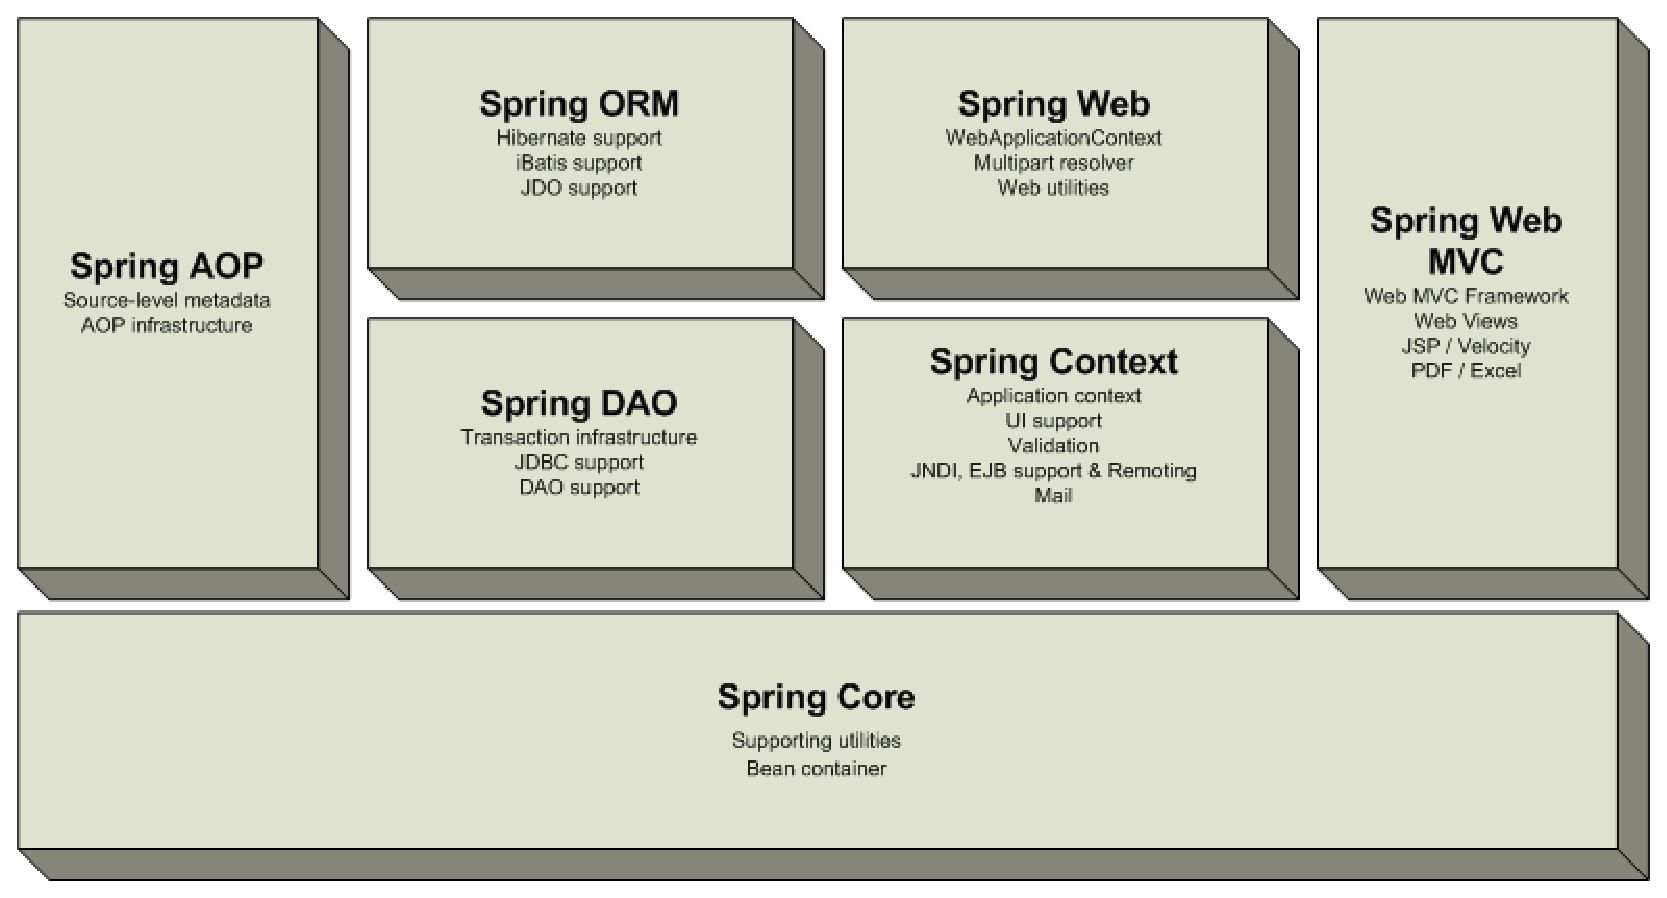
\includegraphics[width=15cm,height=7.9cm]{../images/finalreport/spring-overview.eps}
 \caption{Spring Framework Modules}
\end{figure}

ACE uses the \emph{Core}, \emph{Context}, and \emph{AOP} modules. The
\emph{Core} module provides the most fundamental part of \emph{Spring}, which
is the \emph{Dependency Injection} feature. The basic concept is the
BeanFactory, which removes the need for programmatic singletons. Further, it
allows to remove the tedious \emph{wiring} of the whole application, which
is usually found in applications. For in depth information about
the concept of dependency injection visit the following URL:

\begin{itemize}
 \item \href{http://martinfowler.com/articles/injection.html}{http://martinfowler.com/articles/injection.html}
\end{itemize}

The \emph{Context} module extends the \emph{Core} module by providing access
to internationalization features and application event propagation.

The Spring \emph{AOP} module provides an aspect-oriented programming 
implementation, which is compliant with interfaces defined by the 
\emph{AOP Alliance}. For instance it allows to transparently add method
interceptors to any object defined in the \emph{Spring} context. This allows
to implement so-called cross-cutting concerns, which tend to clutter the
core business logic.


\subsection{Simple Examples}

The \emph{BeanFactory} is one of the core interfaces in \emph{Spring}. It
implements the dependency injection feature. Further, it is the actual
\emph{container} which instantiates, configures, and manages a number of
objects. These objects, called beans in Spring terminology, typcially have
dependencies to other objects also defined in the container. Bean factories
are represented by the \texttt{org.springframework.beans.factory.BeanFactory}
interface. There are several implementations for that interface. However,
usually most applications rely on the \emph{ApplicationContext} interface, which
extends the \texttt{BeanFactory} interface.

\begin{verbatim}
ApplicationContext context = new ClassPathXmlApplicationContext("context.xml");
\end{verbatim}

The passed in \emph{String} points to a resource on the classpath (in this 
case). The \texttt{context.xml} file is an XML file with the following
structure:

\small{\begin{verbatim}
<?xml version="1.0" encoding="UTF-8"?>
<!DOCTYPE beans PUBLIC "-//SPRING//DTD BEAN//EN" 
          "http://www.springframework.org/dtd/spring-beans.dtd">
<beans>
  
  <bean id="..." class="...">
    ...
  </bean>
  <bean id="..." class="...">
    ...
  </bean>

  ...
</beans>
\end{verbatim}}

The top-level \emph{beans} element contains an arbitrary number of \emph{bean}
sub-elements which represent objects managed by the \emph{Spring} container.
In the most common case, the beans are created through constructors. The
\texttt{id} of a bean is a unique identifier of a managed bean in the 
\emph{Spring} container. The \texttt{class} argument specifies the class
of the object to be created. So the following creates a managed bean
with the id \emph{exampleBean} of type \texttt{ExampleBeanClass}:

\small{\begin{verbatim}
  <bean id="exampleBean" class="ExampleBeanClass"/>  
\end{verbatim}}

\emph{Spring} can inject dependencies either through
constructor arguments or through Java Beans properties. Constructor arguments
are specified with the \emph{constructor-arg} child element.

\small{\begin{verbatim}
  <bean id="exampleBean" class="ExampleBeanClass">
    <constructor-arg><ref bean="otherBean"/></constructor-arg>
  </bean>
  
  <bean id="otherBean" class="OtherBeanClass"/>
\end{verbatim}}

Properties of a bean are set through standard Java Beans property set methods.

\small{\begin{verbatim}
  <bean id="exampleBean" class="ExampleBeanClass">
    <property name="collaborator"><ref bean="otherBean"/></property>
  </bean>
  
  <bean id="otherBean" class="OtherBeanClass"/>
\end{verbatim}}

This is just a very coarse-grained overview over \emph{Spring}. For more
details check the excellent documentation available at the following
URL.

\begin{itemize}
 \item \href{http://static.springframework.org/spring/docs/1.2.x/reference/index.html}{http://static.springframework.org/spring/docs/1.2.x/reference/index.html}
\end{itemize}


\subsection{Advantages of Spring}

Using \emph{Spring} in an application has several advantages. We have a look
at some of these in the following sections.

\begin{itemize}
 \item design to interfaces
 \item improved testability
 \item less wiring code
\end{itemize}

\subsubsection{Design to Interfaces}
Spring encourages to split objects into an interface and an implementation.
This helps to clearly specify the methods that are needed to be exposed to
other objects. Further, interfaces provide the possibility to use completely
different implementations of the interface, which is especially useful in
case of testing.

\subsubsection{Improved Testability}
In a typical application, the \emph{Service Locator} pattern is used, which
consists of a singleton \emph{Service Locator}. This service locator provides
access to all the services needed in the application. The use of the singleton
pattern makes it close to impossible to unit test certain parts of the
application.

The availability of interfaces for most business objects as well as the
managed singletons of the \emph{Spring} container give us the possibility
to use \emph{Mock} objects as well as \emph{Stubs} to test our services
in isolation.

\subsubsection{Less Wiring Code}
In a mid-sized application there is a large amount of wiring code. The whole
object graph has to be set up. This wiring code is both tedious and
error-prone. \emph{Spring} removes the wiring process from the application
code into the framework. This might not seem a big deal, but after some time
using it, it becomes evident how much time can be saved.

It must be noted, that all the \emph{magic} done by \emph{Spring} could be
done by hand in the main method of the application. With \emph{Spring} all
this dirty hand-coded wiring of dependencies can be replaced by a 
declaration of all the dependencies in a clean XML file.


\section{BEEP Core}


\section{Bonjour}


